

\vspace{2cm}

Das Robot Operating System (ROS) , ist eine Middleware um flexible Robotik Software zu schreiben. 2007 begann Willow Garage mit der Entwicklung von ROS und findet Heute in der Robotik Community weit verbreitet.
 Es liefert eine Ansammlung von Tools, Libraries und Konventionen, welche das Erstellen von komplexer und robuster Robotik Software auf verschiedenen Platformen erleichtern soll.
ROS gliedert die Algorithmen zur Realisierung intelligenter Roboter in einzelne Aufgaben, welche durch jeweils einen Prozess ( Node ,  Knoten ) dargestelt und auf mehrere Rechner ( Hosts ) verteilt sein können.
Die Nodes verbinden sich nach dem Publisher-Subscriber Schema über ein Netzwerk miteinander um die Datenflüsse herzustellen ( ROS Graph ).
Diese Grafen können aber sehr komplex werden.

\begin{figure}[H]
\centering
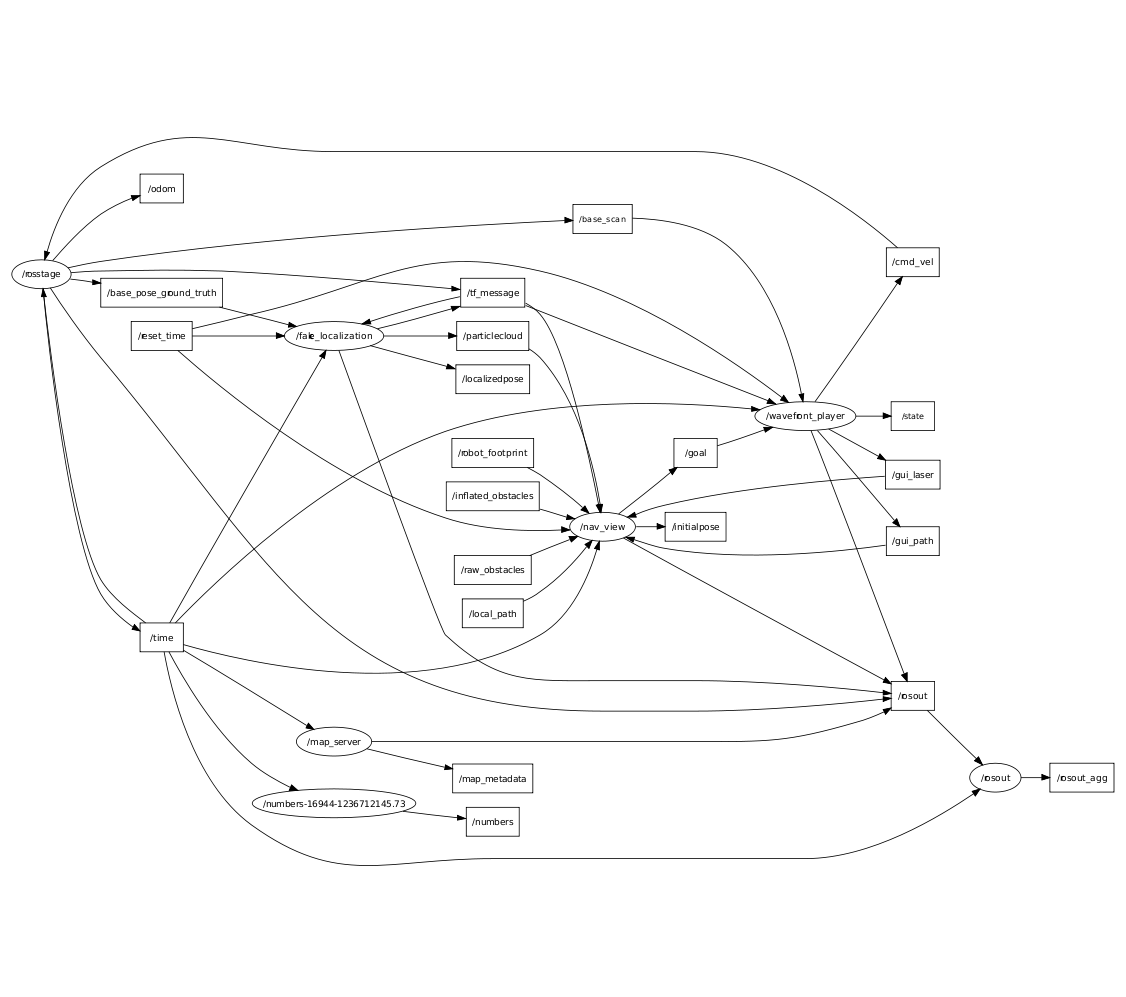
\includegraphics[scale=0.25]{./bilder/rxgraph.png} 
\caption{Beispiel eines ROS Graph. Nodes sind als Ellipsen, Topics als Rechtecke und Datenfluss als Pfeile dargestellt
		Quelle: http://www.willowgarage.com }
\end{figure}

Ein Problem stellt aber die Überwachung dieses Systems dar. Zwar besteht im Moment die Möglichkeit das Gesamtsystem auf Fehler zu überprüfen, aber es nicht möglich zu bestimmen 
welcher Knoten sich fehlerhaft verhaltet. Dies kann besonders bei großen System mit hunderten von Knoten zum Problem werden. Um ein schnelles Debuggen zu ermöglichen, benötigt es
eine Software zum dezentralen Erfassen.


\vspace{0.5cm}

Unser Ziel als PSE-Team ist es, ein System zur Definiton des Soll-Zustandes und der Überwachen des Ist-Zustandes individueller Knoten zu erstellen.